 \begin{center}
 \textbf{
 %\dots
\og 
Vive l’été aux couleurs de la mission !
 \fg{}
 %\dots
 }
 \end{center}

C’est un impératif pour nous de savoir prendre des vacances pour permettre au corps de se refaire. En effet, après un temps de travail, voici venir les jours de décontractions. Le plaisir de ne penser à rien, de se reposer, de profiter de sa famille et de tout ce que l’on aime. Les vacances sont une source de joie, de repos, d’exotisme, de découvertes…On a tous hâte de partir vers de nouveaux horizons ! On se dit même que les vacances sont le meilleur moment pour se ressourcer, pour découvrir de nouveaux lieux et passer du bon temps en famille. Recevoir un petit message de nos proches ou de nos collègues, et surtout de notre curé fait toujours plaisir avant le grand départ en vacances. 

Mais quel message de la part du curé à ses fidèles pendant cette période estivale ? Son message est simple. Il s’agit pour lui de souhaiter de belles vacances dans la paix et la joie à ses fidèles.
Cependant le chrétien en vacances ne devrait pas perdre de vue l’essentiel : le vécu de sa foi en tant que missionnaire comme nous le stipule l’Évangile de ce dimanche. La mission est l’envoi de tous vers tous. En effet, suivre Jésus a pour conséquence d’être envoyés témoigner de lui auprès de nos contemporains.
Cette mission, est elle aussi exigeante et radicale, dans un monde où la bonne nouvelle n’est pas toujours accueillie favorablement. C’est en cela que, l’évangélisation n’est l’affaire d’une catégorie de personnes, mais elle est l’œuvre de l’Église ; aussi bien des prêtres, religieux et religieuses que des laïcs, dans toute sa composante : enfants, jeunes et adultes.
Tous appelés, tous missionnaires.

\begin{wrapfigure}{l}{1.0cm}
\vspace{-0.4cm}
	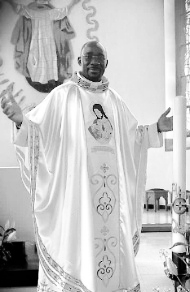
\includegraphics[scale=1.20]{../images/standing_daniel}
\end{wrapfigure}
Il est important de le rappeler avec abnégation qu’un chrétien qui n’est pas missionnaire est démissionnaire. Car c’est à la capacité de communiquer la foi reçue au baptême que se mesure la maturité de l’adhésion au Christ.
Pendant toute cette période estivale, profitons véritablement de nos vacances mais n’oublions pas que Dieu n’est pas en vacances. Partout où nous serions, au bord des plages, dans les cathédrales, dans nos églises et même dans nos chapelles, ouvrons à Dieu nos cœurs afin qu’il y habite pour qu’en chaque occasion, nous reconnaissons ses œuvres pour lui dire merci. Que cet été soit pour nous un temps favorable à la louange du Créateur à travers toutes ses bienfaits.

\begin{flushright}
Bel été à toutes et à tous !!!
\textit{Père  Daniel  ETTÉ}
\end{flushright}

